\documentclass{standalone}
\usepackage{tikz}

\tikzset{XOR/.style={draw,circle,append after command={
			[shorten >=\pgflinewidth, shorten <=\pgflinewidth,]
			(\tikzlastnode.north) edge (\tikzlastnode.south)
			(\tikzlastnode.east) edge (\tikzlastnode.west)
		}
	}
}



\begin{document}

			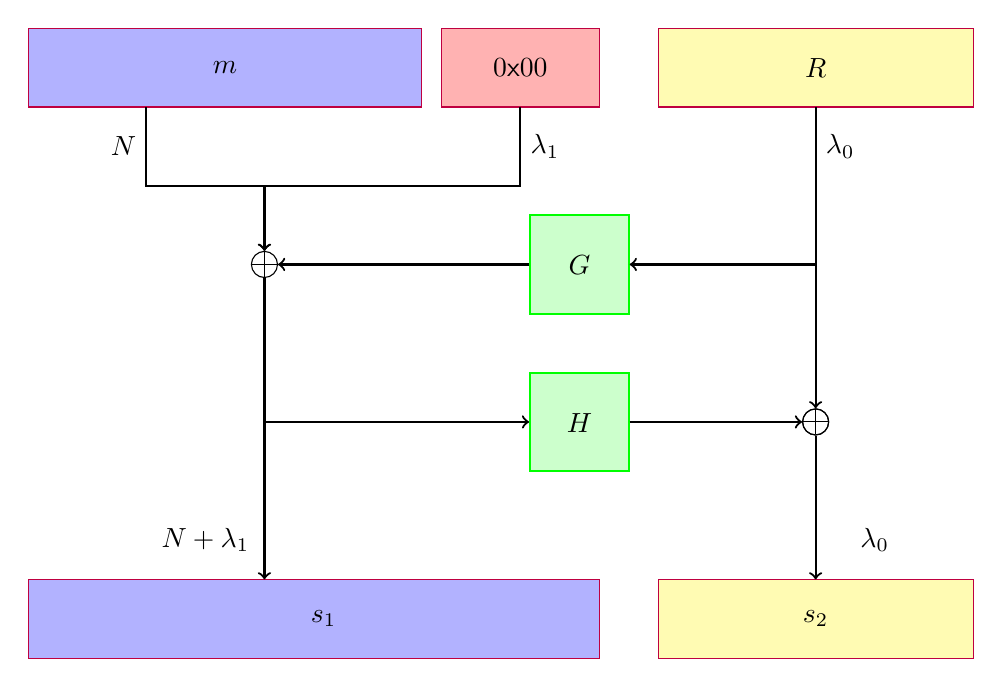
\begin{tikzpicture}
				\tikzstyle{SQUA} = [thick, minimum width=1.25cm, minimum height =1.25cm, text height=2ex, text depth=0.25ex]
				\tikzstyle{key} = [RECT, draw=green, fill=green!20]
				\tikzstyle{prf} = [SQUA, draw=green, fill=green!20]
				
				\draw [fill=blue!30,draw=purple] (1,0) rectangle (6,1);
				\node [] at (3.5,0.5) {$m$};
				\draw [fill=red!30,draw=purple] (6.25,0) rectangle (8.25,1);
				\node [] at (7.25,0.5) {$0\mathsf{x}00$};
				\draw [fill=yellow!30,draw=purple] (9,0) rectangle (13,1);
				\node [] at (11,0.5) {$R$};
				
				\node[XOR] (xor1)  at (4,-2) {};
				\draw[->,thick] (2.5,0) -- (2.5,-1) node [midway,left] {$N$} -| (xor1.north) ;
				\draw[->,thick] (7.25,0) -- (7.25,-1) node [midway,right] {$\lambda_1$} -| (xor1.north) ;
				
				\node[prf] (G)     at (8, -2) {$G$};
				\draw[->,thick] (11,0) -- (11,-1) node [midway,right]   {$\lambda_0$} |- (G.east);
				\draw[->,thick] (G.west) -- (xor1.east);
				
				\node[prf] (H)     at (8, -4) {$H$};
				\draw[->,thick] (xor1.south) |- (H.west);
				
				\node[XOR] (xor2)  at (11,-4) {};
				\draw[->,thick] (11,0) -- (xor2.north);
				\draw[->,thick] (H.east) -- (xor2.west);
				
				\draw [fill=blue!30,draw=purple] (1,-7) rectangle (8.25,-6);
				\node [] at (4.75,-6.5) {$s_1$};
				\node[XOR] (xor2)  at (11,-4) {};
				\draw[->,thick] (xor1.south) -- (4,-6);
				\node [] at (3.25,-5.5) {$N+\lambda_1$};
				\draw [fill=yellow!30,draw=purple] (9,-7) rectangle (13,-6);
				\node [] at (11,-6.5) {$s_2$};
				\draw[->,thick] (xor2.south) -- (11,-6);
				\node [] at (11.75,-5.5) {$\lambda_0$};
				
			\end{tikzpicture}
\end{document}
